% !TEX root = ../../thesis.tex

\section{Numerical Example}\label{sec:example}
We focus on the New England power system comprising 10 generators and 39 buses, and simulate the system for $t=20$ seconds \textcolor{black}{with a discretization step of $1/60$ seconds}. The values of the system parameters are taken from \cite{new_england1}-\!\!\cite{new_england2}. The power system is running under normal condition from $t=0$ to $t=2$ seconds. \textcolor{black}{At $t=2$ seconds, a three-phase fault occurs at Bus 17. Then, Line 17�-18 is tripped out to clear the fault. However, the WACS is unaware of this fault at this time. Two seconds later, at $t=4$ seconds, the WACS detects the occurrence of this fault, i.e., there is a $2$~second-delay in the WACS being able to respond to the fault.} We conduct load flow analysis of the power system before and after the occurrence of the 3-phase fault, to find the values of $P_{i}^e$, $ \theta_i$, and $|E_i|$ for each generator. We demonstrate the effectiveness of our proposed secure estimation method through simulations of 3 different scenarios:
%\textcolor{black}{Do we have to explain what Line 17--18 is or is it obvious?}\textcolor{black}{I think it is clear that we are focusing on the New England system.}
\begin{enumerate}
\item \textit{Scenario 1:} There is no simultaneous cyber attack on the power system.
\item \textit{Scenario 2:} The power system is also under cyber attack, and it is not protected by secure estimation.
\item \textit{Scenario 3:} The power system is also under cyber attack, and it is protected by secure estimation.
\end{enumerate}

The plots titled ``No Attack'' in Fig.~\ref{fig:SE} show the simulation results of Scenario 1: an attack-free power system under a three-phase fault. For clarity, only phase angles and rotor speeds of generators 1, 2 and 3 are shown in Fig.~\ref{fig:SE}. At $t=0$ seconds, the system is under equilibrium, all ten generators' rotor speeds are at the nominal value, $\omega_0$, of 60~Hz, and their phase angles are $6.85^\circ, 5.09^\circ, 6.28^\circ, 8.81^\circ, 7.38^\circ, 11.30^\circ, 14.74^\circ, 8.35^\circ, 7.63^\circ$ and $-13.11^\circ$, respectively. At $t=2$ seconds, a three-phase fault occurs at Bus 17 which causes a change in the line admittances ($y_{ij}$'s and $\phi_{ij}$'s) and consequently, the total active power leaving bus $i$, $P^e_i$. However, the WACS is unaware of this fault until $t=4$ seconds. \textcolor{black}{During this 2~second-delay, the WACS is unaware of the fault and continues to use the pre-fault line admittance values in the secure estimation algorithm. The local controllers at the generators continue to compute the control input $U_i$ using the received measurements from the WACS, which leads to a mismatch between $P^e_{i,\text{meas}}$ and $P^e_i$, and causes the phase angles and rotor speeds of the generators to deviate from their equilibrium. At $t=4$ seconds, the WACS becomes aware of the fault. It computes the new line admittance values under this fault, and uses the new line admittance values in the secure estimation algorithm. The local controllers then use the received estimates to compute the local control input $U_i$, making $P^e_{i,\text{meas}} = P^e_i$ again.} As a result, the generators' rotor speeds slowly converge back to 60~Hz and their rotor angles settle at new equilibrium values.



In Scenarios 2 and 3, in addition to the 3-phase fault, the power system is also subject to the following cyber attack. Malicious attacks targeted at generator 1 are injected from $t = 0.33$~seconds onwards. A set of 10 measurements that varies with time are corrupted. More specifically, at each time step, the attacker randomly chooses to perform either a c-attack or an m-attack.
In the case of a c-attack, the attacker corrupts phase angle measurements that generator 1 receives from all its 9 neighbors (i.e., $y^c_{1,2}, y^c_{1,3}, \ldots, y^c_{1,10}$) with independent Gaussian signals from the distribution $\mathcal{N} (0, 180^\circ)$. In addition, a constant signal of $90^\circ$ is injected into the measurement $y^c_{1,2}$.
In the case of an m-attack, the attacker randomly chooses 9 measurements from the set of 10 measurements that generator 1 submits to the WACS $(i.e., y^m_{1,1}, y^m_{1,2}, \ldots, y^m_{1,10})$, and corrupts each chosen measurement with an independent Gaussian signal from $\mathcal{N} (0, 180^\circ)$. Similarly, an additional constant signal of $90^\circ$ is injected into the measurement $y^m_{1,2}$.
%\textcolor{black}{Do we need the constant attack? It would be better to put an explanation.}
The left plot in Fig.~\ref{fig:attack} shows the true attack signals. Rows 1 to 9 correspond to c-attacks: $e^c_{1,2}, e^c_{1,3}, \ldots, e^c_{1,10}$, and rows 10 to 19 correspond to m-attacks: $e^m_{1,1}, e^m_{1,2}, \ldots, e^m_{1,10}$. Since constant signals of $90^\circ$ are injected on top of the Gaussian attacks to $y^c_{1,2}$ or $y^m_{1,2}$ for c-attacks or m-attacks, respectively, the mean attack signals are higher for row 1 (i.e., $e^c_{1,2}$) and row 11 (i.e., $e^m_{1,2}$). For clarity, the measurements that are not attacked during the simulation are not shown.


In Scenario 2, no secure estimation-based protection is implemented. Therefore, when the system is under cyber attack, the local controller at generator 1 computes $P^e_{1,\text{meas}}$ using corrupted measurements, causing $P^e_{1,\text{meas}} \neq P^e_1$.
As a result, the feedback control law in (\ref{Eq:Ui}) fails to linearize the system dynamics (\ref{swing2k}).
The constant signal of $90^{\circ}$ injected on top of the Gaussian attacks causes oscillations in the rotor speed of generator 1 due to the sine term in its dynamics (refer to Eq.~(\ref{Eq:Ui}) to (\ref{Eq:yc})). The oscillations in the rotor speed then leads to oscillations in generator 1's rotor angle.
The plots titled ``Under Attack, no SE'' in Fig.~\ref{fig:SE} show that these oscillations are observed on top of the system's response to the 3-phase fault, and prevents generator 1's phase angle to reach a new equilibrium even after the fault has cleared.
In addition, the cyber attack causes larger differences in other generators' equilibrium rotor angles before and after the fault. For example, in Scenario 1, when there is no cyber attack, generator 2 and 3's rotor angles after the fault are $-14^{\circ}$ and $-8^{\circ}$ respectively. On the other hand, in Scenario 2, their post-fault equilibrium rotor angles are $-25^{\circ}$ and $-17^{\circ}$ respectively.


%This causes generator 1's rotor speed to deviate from the nominal value, which in turn, causes the generator's rotor angle to rapidly diverge from its equilibrium value, reaching $159^\circ$ within 7.3~sec, as shown in the left plots in Figure \ref{fig:SE}. When the phase angle difference between two generators exceeds $90^\circ$, the generators can potentially loose synchrony and trip. In this simulation, the phase angle difference between generators 1 and 10 exceeds $90^\circ$ at 4.78~sec.
%As shown in Fig. \ref{fig:attack}, the proposed state estimation enables the WACS to reconstruct the rotor angles and rotational speeds of the generators accurately, and to prevent all possible failures.





\begin{figure}
\centering
%\vspace*{-0.3cm}
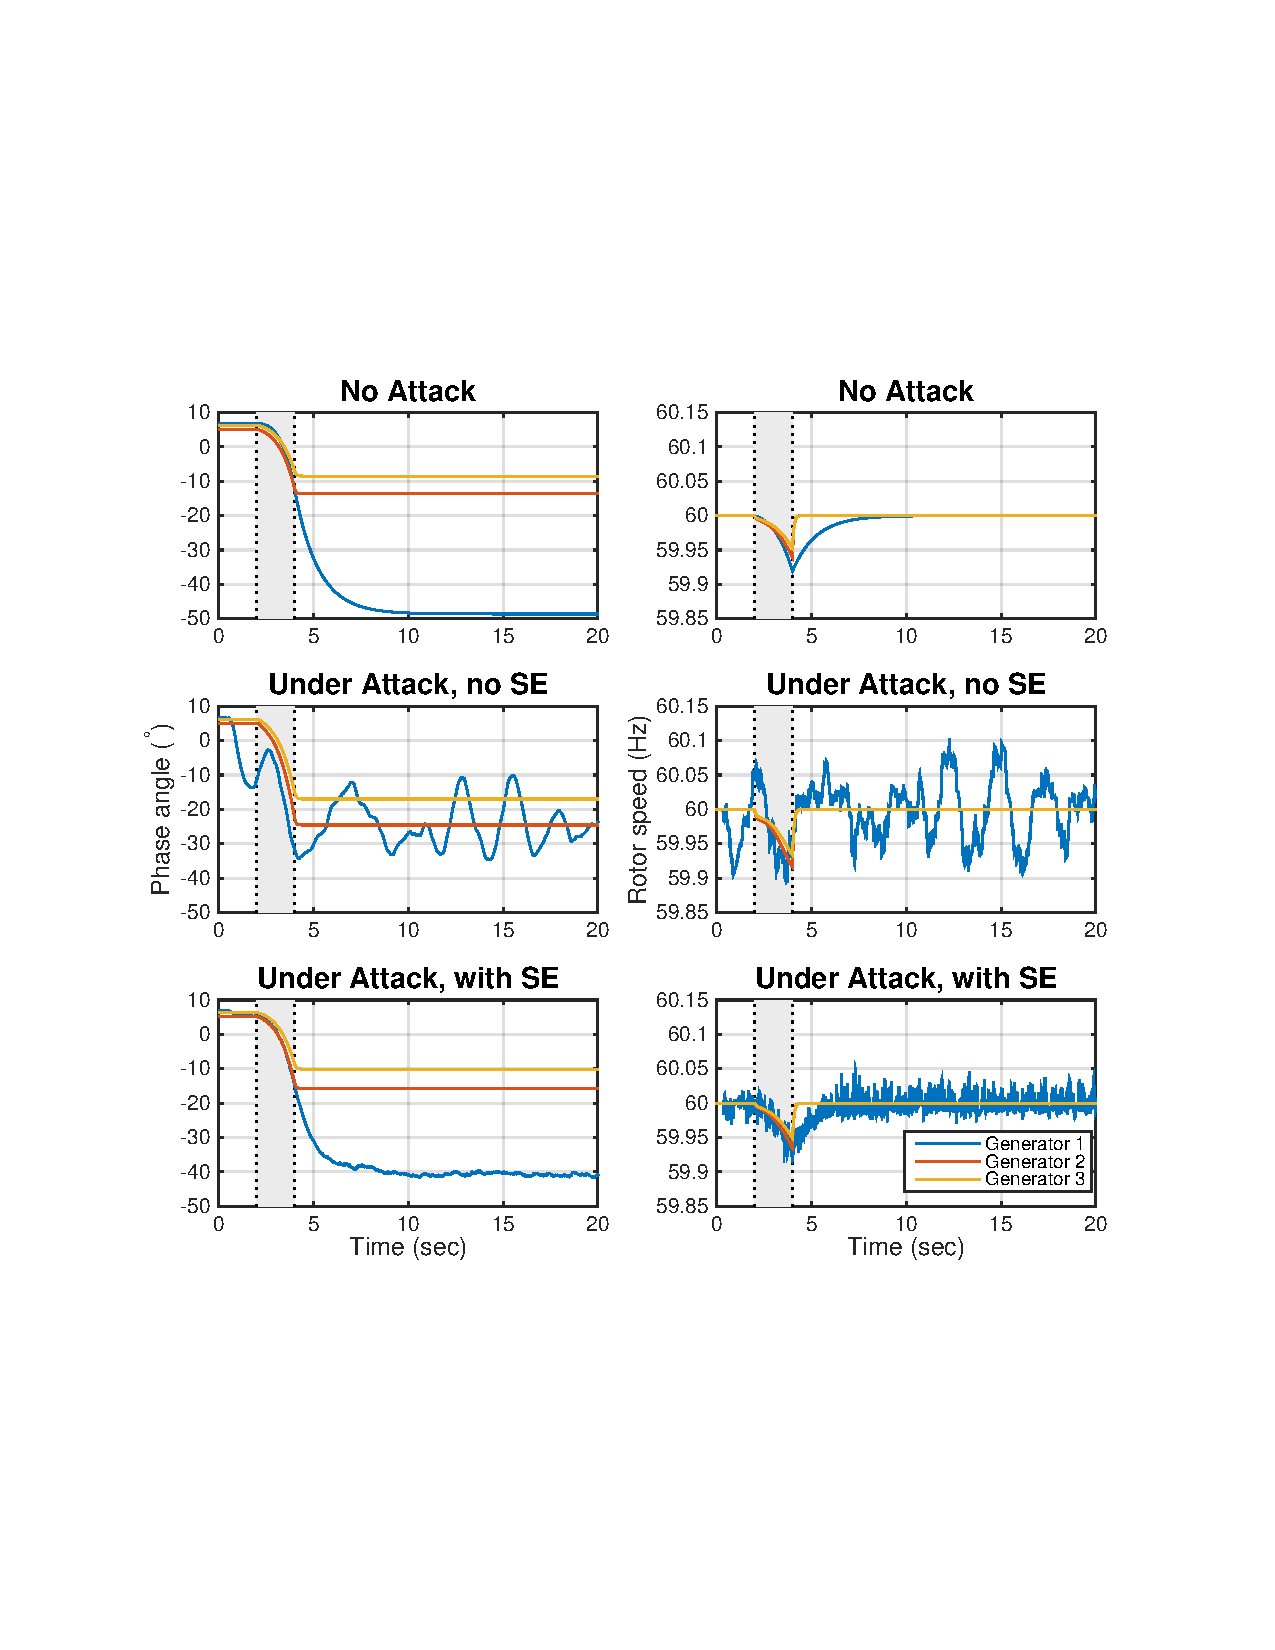
\includegraphics[scale=0.5]{chapters/se_nonlinear/figures/SE3.pdf}
%\vspace*{-0.8cm}
\caption{Evolution of phase angles and rotor speeds of generators 1, 2 and 3 under a 3-phase fault, in three scenarios: (1) there is no attack, (2) system is under attack and there is no secure estimation (SE), (3) system is under attack and WACS uses SE. Fault happens at $t=2$ seconds. Grey region marks the 2 seconds delay in WACS being informed of the fault. In (2), cyber attack causes generator 1's rotor angle and speed to oscillate. In (3), incorporating SE damps the large oscillations and makes the system's response more closely resemble that of (1).}
\label{fig:SE}
\end{figure}

\begin{figure}
\centering
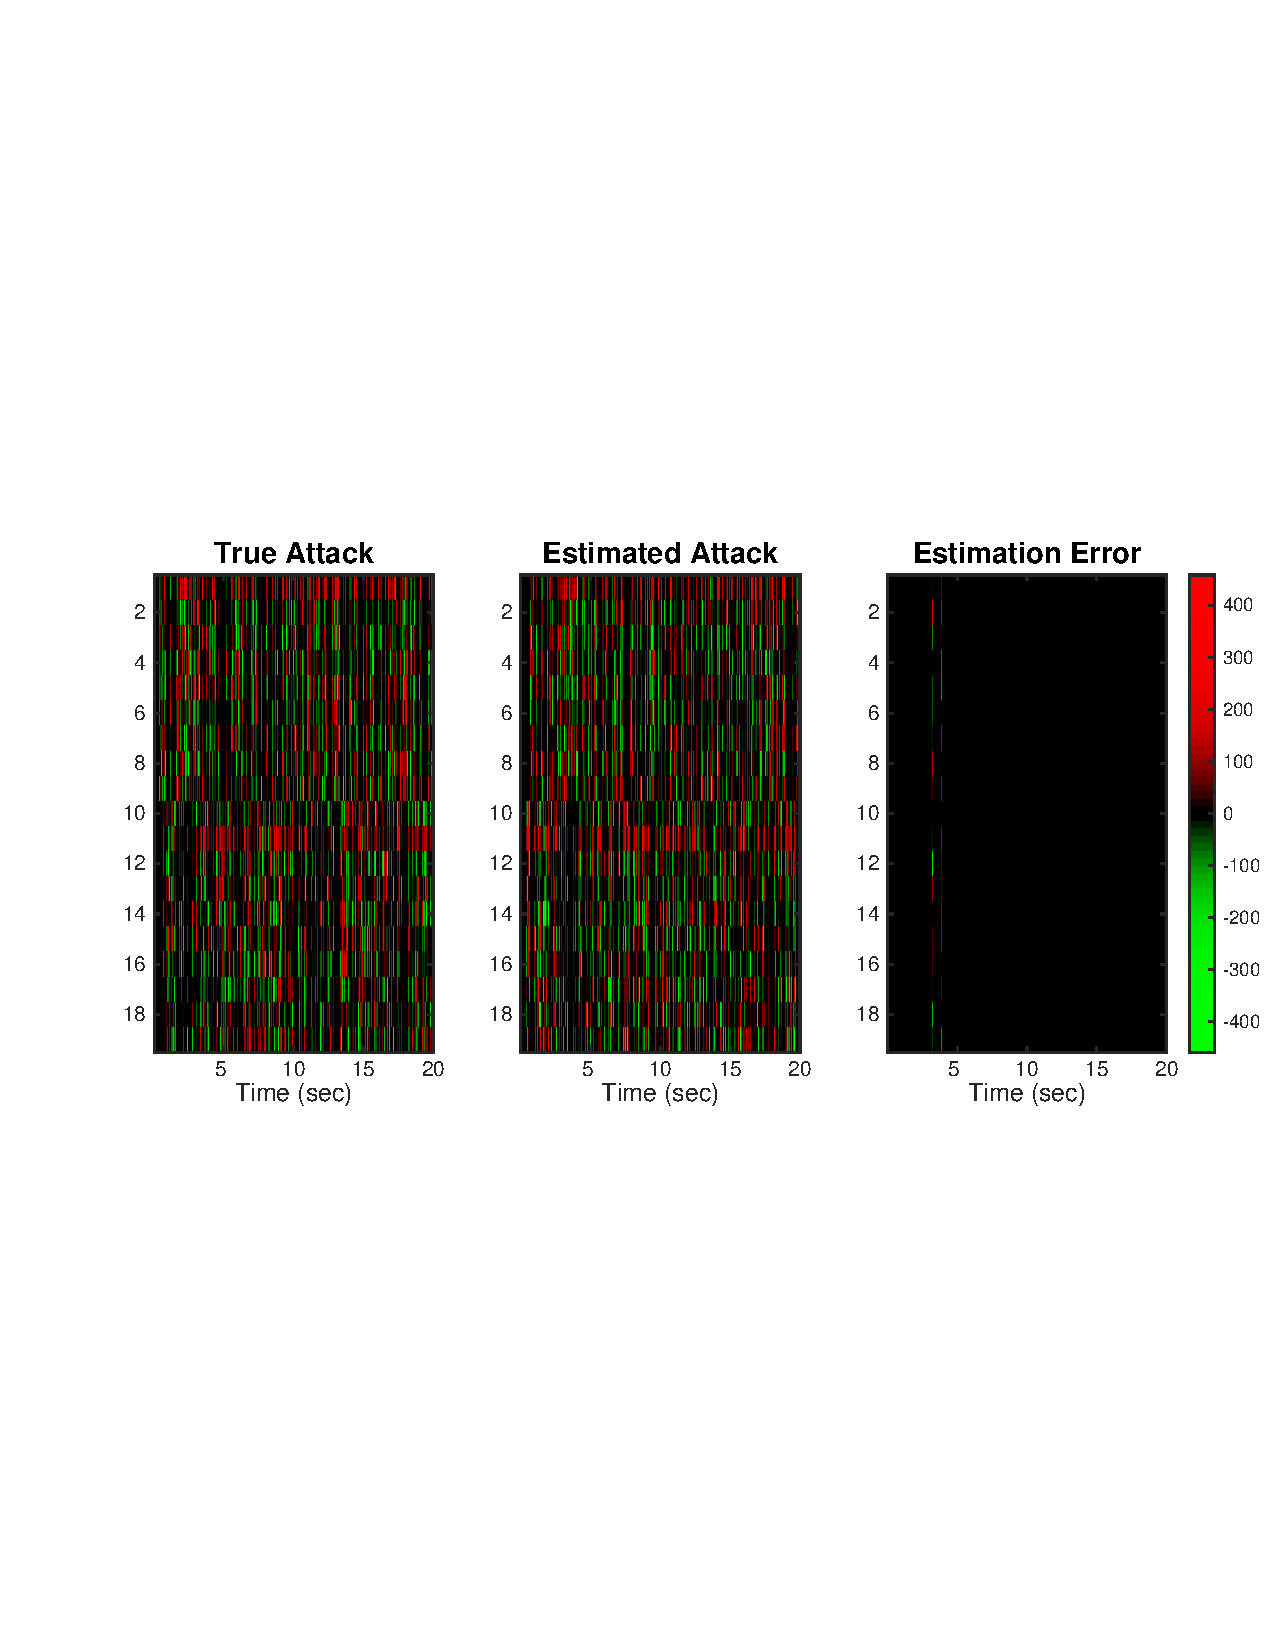
\includegraphics[scale=0.42]{chapters/se_nonlinear/figures/attack.pdf}
%\vspace*{-0.5cm}
\caption{True and estimated attack signals: The rows and columns correspond to attacked measurements and time steps, respectively. In subfigures ``True Attack'' and ``Estimated Attack'', the color indicates the attack signal: red is a positive attack, green a negative attack, and black is no attack. In subfigure ``Estimation Error'', the black color indicates there is zero estimation error for all measurements at all times.}
%\vspace*{-0.3cm}
\label{fig:attack}
\end{figure}


Finally, in Scenario 3, the power system is subject to the same cyber attack as in Scenario 2. However, the WACS uses secure estimation to protect the system against such attacks.
The center and right plots in Fig.~\ref{fig:attack} show the secure estimator's estimated attack signal and the estimation error respectively.
The results show that the secure estimator correctly estimates the attack signal before the fault happens at $t=2$ seconds. Between $t=2$ and $t=4$ seconds, there are small estimation errors due to model mismatch as the WACS is unaware of the fault and continues to use the pre-fault line admittance values in the secure estimation algorithm. However, once the WACS is informed of the fault at $t=4$ seconds, the model mismatch is removed and estimation error is cleared. The estimated the attack signals are then subtracted from the corrupted measurements to recover the true rotor angles and speeds. The reconstructed measurements are communicated to all generators, and used to compute $P^e_{1,\text{meas}}$. By doing this, the local controllers obtain a value of $P^e_{1,\text{meas}}$ that is a more accurate estimate of the true $P^e_1$ than when no secure estimation was used.
The bottom plots, titled ``Under Attack, with SE'', in Fig.~\ref{fig:SE} show the rotor angles and speeds of generators 1, 2, and 3 in this scenario.
Observe that throughout the simulation, generator 1's rotor angle is much more stable in this scenario than in Scenario 2.
In addition, note that when the power system is under cyber attack, the behavior of the system with secure estimation (Scenario 3) resembles more closely the system's behavior when there is no cyber attack (Scenario 1), than the system without secure estimation (Scenario 2) does.


As mentioned earlier, there is a 2-step estimation delay in the proposed secure state estimator. Our numerical results show that this estimation delay will not affect the phase angle and rotor speeds significantly. This can be explained by the fact that the attack signals effect on the system dynamics are scaled
by the matrix $H$ (see equations (26) and (27)) whose entries are very small due to the small discretization time step (1/60 seconds) and the large generators' inertia (i.e., attack signals cannot immediately have a significant effect on the generators' phase angles and speeds).
\textcolor{black}{The simulation was repeated using a larger discretization time step of 1/30 seconds and the same observations were made (the control feedback gain $F_i$ was adjusted accordingly). Due to space limitations, we do not show the results here.}

